\documentclass[11pt]{article}
\usepackage{acl2014}
\usepackage{times}
\usepackage{url}
\usepackage{latexsym}
\usepackage{float}
\usepackage{graphicx} 
\usepackage{subfigure}

%\setlength\titlebox{5cm}

\title{Gender and Facial Expression Classification}

\author{Jifu Zhao\\
  Graduate Student\\
  Department of Nuclear, Plasma, and Radiological Engineering \\
  {\tt jzhao59@illinois.edu} \\}

\date{\today}

\begin{document}
\maketitle

\section{Introduction}

Picture is an important way for human to communicate with the world. Especially now, with the development of modern social media, such as Facebook, Twitter, Instagram and so on, people tend to express their emotions through social media. With so many information online, it is needed to make the machine to learn how to classify the pictures based on gender, facial expressions and so on. This will be helpful to improve the experience of social media.\\

In this paper, we will address the very simple problem: given a collection of pictures, how to make the computer correctly classify the gender and facial expression.\\

This proposal will be divided into the following sections. Section 2 describes the dataset and problem to be solved. Section 3 will talk about the methods that will be used in this paper. Finally, section 4 will talk about the goal for this project.\\

\section{Dataset and Problem}

For this project, we will use th FEI Face Database (Thomaz and Giraldi, 2010). The FEI face database (\url{http://fei.edu.br/~cet/facedatabase.html}) is a Brazilian face database that contains a set of face images for 200 individuals. Including 100 males and 100 females. These pictures is divided into different types based on their information, such as color scale, gray scale, only frontal face images and so on. In this project, we use three subsets of the original images.\\

The first one is the smallest images: only the frontal face images, as shown in Figure 1. \\
\begin{figure}[H]
\centering
\subfigure[Non-smile]{
\label{Fig.sub.1}
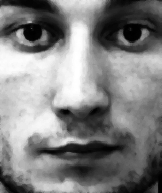
\includegraphics[width=0.2\textwidth]{2alittle.jpg}}
\subfigure[Smile]{
\label{Fig.sub.2}
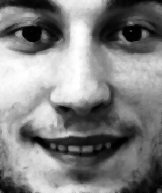
\includegraphics[width=0.2\textwidth]{2blittle.jpg}}
\caption{Frontal faces}
\label{Fig.lable}
\end{figure}

\begin{figure}[H]
\centering
\subfigure[Non-smile]{
\label{Fig.sub.1}
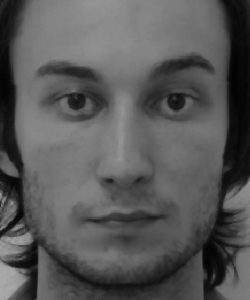
\includegraphics[width=0.2\textwidth]{2afront.jpg}}
\subfigure[Smile]{
\label{Fig.sub.2}
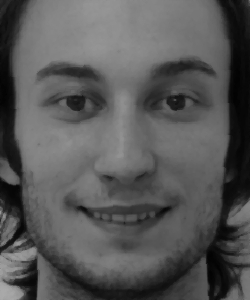
\includegraphics[width=0.2\textwidth]{2bfront.jpg}}
\caption{Full faces}
\label{Fig.lable}
\end{figure}

\begin{figure}[H]
\centering
\subfigure[Non-smile]{
\label{Fig.sub.1}
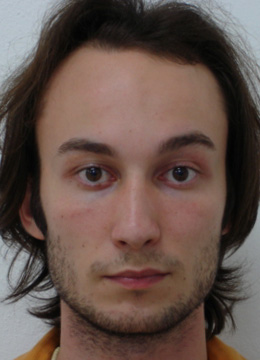
\includegraphics[width=0.2\textwidth]{2a.jpg}}
\subfigure[Smile]{
\label{Fig.sub.2}
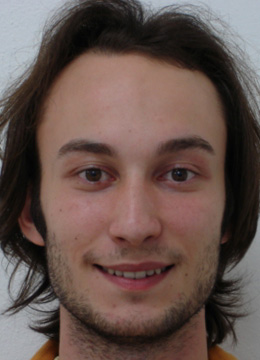
\includegraphics[width=0.2\textwidth]{2b.jpg}}
\caption{Colored faces}
\label{Fig.lable}
\end{figure}

The second one is also the gray scale images, but this time there will be more information, such as hair. The sample picture is shown in Figure 2.\\

And the third subset, which contains the images in RGB format, contains all the information.\\

There will be 400 images in each subset, and 200 individuals with smile expressions and the other 200 individuals with non-smile expressions. So, for each subset, there will be 100 men with smile expression, 100 men without smile expression, 100 women with smile expression, 100 women without smile expression. Using these 400 images, we can do a lot of work. But, in this project, we will try to solve the following problem:\\

Given the training images, how much information do we need to correctly classify the images into male and female, smile and non-smile classes.\\

\section{Methodology}

In this project, the we need to deal with the images. The method to be used in this project is that: we will transfer every image into one column vector. So, every pixel will be looked as one feature. In those three subsets, the feature number will be:

\begin{center}
$193 \times 162 = 31266$\\
$300 \times 250 = 75000$\\
$360 \times 260 \times 3 = 280800$\\
\end{center}
Using 280800 features is not realistic, so the first thing we need to do is the reduce the dimensionality. The method to be used will be {\bf Principal Component Analysis (PCA)}.\\

Through PCA method, we can reduce the original dimensionality from more than 30000 features into even several components. In this we, we only need to consider these several components.\\

Ideally, we hope that the dimensionality can be reduced into less than 4 dimensions. Because in this way, it is much easy for us to visualize our data.\\

After reducing the dimensionality, we will do classification in the new space. To successfully classify the pictures based on the features, we will first use linear classifiers, then try more complex classifiers. Currently, we plan to use the {\bf Perception}, {\bf Quadratic Discriminant Analysis}, {\bf Support Vector Machines (SVM)}, {\bf k-Nearest Neighbors (k-NN)} and so on.\\

\section{Project Goal}

The goal of this project are separated into three parts. The first goal is to learn to apply different machine learning methods into real problems. This should also be the goal of this course. We hope to show that we truly learn something from this class.\\

The second goal is that: show the relation between the information given and the conclusion that can be concluded. In this project, we want to see in order to correctly classify the gender and facial expression only based on the images given, how much information do we need. Our expectation is that, based on the first subset of images, we can only distinguish the face to be smile or not, because there is only little information contained. But we will evaluate how many dimensions do we need to successfully classify them. Maybe only one dimension will be enough, maybe more. For the second and third subset of images, we hope to successfully classify gender and facial expressions and also, compare different classification methods based on their accuracy. \\

Those are just our current goal. In the future, we may add more goals and use more complex models, such as face recognition and so on. We hope to imply the algorithm into the real-world problems. This project may looks simple, but it is a good start for us to apply what we learn.

\begin{thebibliography}{}

\bibitem[\protect\citename{Thomaz and Giraldi}2010]{Aho:72}
C. E. Thomaz and G. A. Giraldi.
\newblock 2010.
\newblock {\em A new ranking method for Principal Components Analysis and its application to face image analysis}, volume~28.
\newblock Image and Vision Computing.

\bibitem[\protect\citename{Theodoridis and Koutroumbas}2009]{Aho:72}
S. Theodoridis and K. Koutroumbas
\newblock 2009.
\newblock {\em Pattern Recognition (Fourth Edition)}, 
\newblock Elsevier Inc.

\bibitem[\protect\citename{Theodoridis and Koutroumbas}2009]{Aho:72}
M. A. Turk and A. P. Pentland
\newblock 1991.
\newblock {\em Face Recognition Using Eigenfaces}, 
\newblock Computer Vision and Pattern Recognition.

\bibitem[\protect\citename{Delac, Grgic and Grgic}2006]{Aho:72}
K. Delac, M. Grgic and S. Grgic
\newblock 2006.
\newblock {\em Independent Comparative Study of PCA, ICA, and LDA on the FERET Data Set}, 
\newblock International Journal of Imaging Systems and Technology.

\end{thebibliography}

\end{document}
